\chapter{Literature Review}
The main purpose of this chapter is to present the needed theoretical and technical background to understand how the plugin works. Therefore, a short but sufficient definition of various concepts and tools will be given. In terms of theoretical context, this chapter will discuss topics like  Event-B, Maude and the rewriting logic approach to Event-B. Furthermore, this chapter will also provide some insight into plugin development in Rodin. To guide the reader through the different sections of this chapter and facilitate their reading, the following section dependency is given:

%insert image of section dependencies


\section{Event-B}
%explain what event B is generally
Event-B \cite{Abrial2011,Butler2013} is a formal method for specifying and verifying properties about systems based on set theory and predicate logic. Specifications in Event-B are referred to as models, and they are semantically modeled by a discrete labeled transition system or LTS \cite{LTS}. The main components of an Event-B model are machines and contexts: machines contain the dynamic elements of the model, while contexts contain the static ones. Specifically, machines contain the system variables, invariants, theorems, variant and events. On the other hand, contexts contain carrier sets, constants, axioms and theorems. Both machines and contexts have different interactions between them. A machine can "see" one or several contexts, meaning that the machine includes the static elements specified in these contexts. Furthermore, machines can "refine" other machines, which means that if a machine $M_2$ refines a machine $M_1$, then $M_2$ can use all the dynamic elements specified in $M_1$ and also create new ones that respect the properties defined in $M_1$ (for example properties defined as invariants). This relation also occurs in the same way between contexts, when one context "extends" another one.
%explain what a Context is and syntax 
In terms of syntax, the general structure for contexts is expressed in figure \ref{fig:eventb2}. The definition for each one of the elements of the syntax is:
\begin{itemize}
    \item \textit{context\_identifier} is a string that identifies the context. The context identifier must be different to all the other identifiers of the components of the system (other machines or contexts).
    \item The "extends" clause lists all the contexts identifiers that the current context is extending.
    \item The "sets" clause takes a list of set identifiers. Each one of these set identifiers correspond to the name of one of the carrier sets of the model. A carrier set is a user defined set or type, that must be non-empty. The set of set identifiers of a model is defined as $\bar{s} = \{s_1...s_n\}$. 
    \item The "constants" clause lists all the constants of the model. The set of constants identifiers is defined as $\bar{c} = \{c_1...c_n\}$.
    \item The "axioms" clause introduces the list of axioms that the model must satisfy. The Axioms are a conjunction logic predicates over sets $\bar{s}$ and constants $\bar{c}$ defined as $A(\bar{s},\bar{c})$. These logic predicates state the properties that the constants and sets must meet.
    \item The "theorems" clause lists some logic predicates, that must be proved within the context using the axioms. These are logic predicates defined as $T_i(\bar{s},\bar{c})$.
\end{itemize}
\begin{figure}[h]
    \centering
    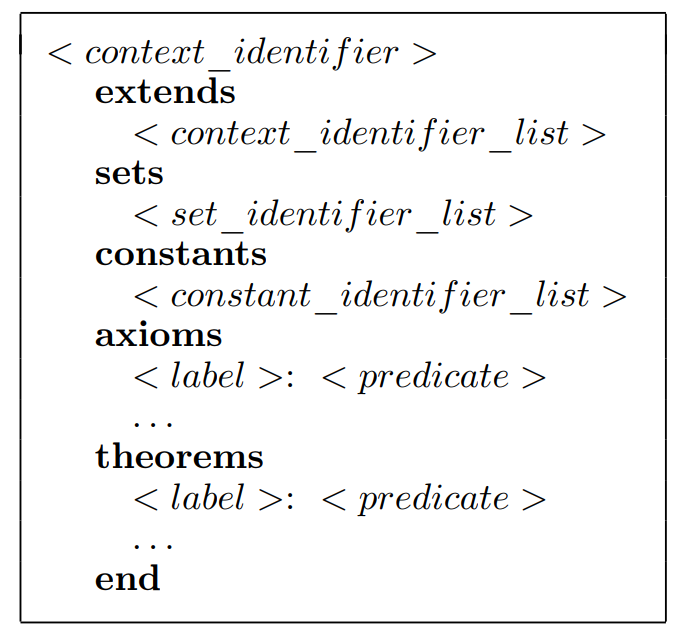
\includegraphics[scale = 0.3]{images/eventb2.PNG}
    \caption{Context structure, taken from \cite{Abrial2011}}
    \label{fig:eventb2}
\end{figure}

%explain what a Machine is and syntax
The general structure of the machine is specified in figure \ref{fig:eventb3}.  
\begin{figure}[h]
    \centering
    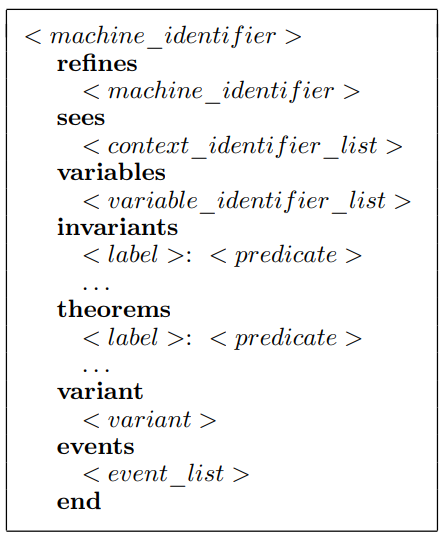
\includegraphics[scale = 0.4]{images/eventb3.PNG}
    \caption{Machine structure, taken from \cite{Abrial2011}}
    \label{fig:eventb3}
\end{figure}
Each one of its components correspond to:
\begin{itemize}
    \item \textit{machine\_identifier} is a string that identifies the machine. It must be different from all the other components identifiers.
    \item The "refines" clause contains the identifier of the machine that this machine refines.
    \item Clause "sees" lists the context that the machine is referencing. When a machine "sees" a context, it means that it can use the sets and constants defined in the context.
    \item The clause "variables" lists all the variables of the system. The set of variable identifiers is defined as $\bar{v} = \{v_1...v_n\}$.
    \item The "invariants" clause lists all the invariants that the model must satisfy. Invariants are represented as a conjunction of logic predicates over variables $\bar{v}$, defined as $I(\bar{v})$. These invariants define the properties that the variables must hold in every configuration or state of the system.
    \item The "theorems" clause lists all the theorems. Each theorem is a logic predicates that must be proven using the axioms of the context and the invariants of the machine. They have the form $T_i(\bar{v})$.
    \item The "variant" clause is used when machines have \textit{convergent events}. It specifies an expression $V(\bar{v})$ over the variables used for proving convergence of the model, i.e. proving that the model doesn't loops forever.
    \item The "events" clause lists the events of the model. Each event represents a system transition, that changes the current system state to another.
\end{itemize}
Events are very important components of an Event-B model and they have the following structure:
\begin{align*}
    \textbf{event} \; e \; \textbf{any} \; \bar{t} \; \textbf{where} \; G(\bar{t}, \bar{v}) \; \textbf{then} \; S(\bar{t}, \bar{v}) \; \textbf{end} 
\end{align*}
\begin{itemize}
    \item $e$ is the \textit{event\_identifier}, which is a string that identifies the event.
    \item The "any" clause lists the parameters of the event. The set of parameters of an event is represented by $\bar{t} = \{t_1,...,t_n\}$.
    \item The "where" clause contains the guards of the event. Guards are represented as a conjunction of logic predicates $G(\bar{t}, \bar{v})$ over the parameters of the event and variables of the system. These guards specify the conditions that must hold for the event to be enabled.
    \item The "then" clause contains the list of actions of the event. Actions define variable assignments that change the variable values when the event is executed. These actions are represented as a set of assignments $S(\bar{t}, \bar{v})$.
\end{itemize} 
%explain what is an action
event assignments can be categorized in three types:
\begin{itemize}
    \item Deterministic assignment $x := E(t,v)$ states that if the event is executed, then the value of variable $x$ in the next model state will be $E(t,v)$, where $E$ is an expression over the parameters of the event and the variables of the system.
    \item Non-deterministic assignment $x :\in  \{ E_1(\bar{t},\bar{v})... E_n(\bar{t},\bar{v}) \}$ called enumerated assignment. In this case, one of the expressions $E_i$ of the set is assigned non-deterministically to variable $x$, when the event is executed.
    \item Non-deterministic assignment $x :\! | \; Q(\bar{t}, \bar{v}, x, x')$ called predicate assignment. It assigns to variable $x$ the value $x'$, s.t. $x'$ satisfies the predicate $Q(\bar{t}, \bar{v}, x, x')$.
\end{itemize}
The set of events of a model is called as $Evts$. This set includes the \textit{INITIALISATION} event or $Init$, which assigns the initial value to all the variables of the machine and creates the initial state of the model. A whole Event-B model can be represented as a context $\mathscr{C} = (\bar{s},\bar{c}, A(\bar{s},\bar{c}))$ and a machine $\mathscr{M} =(\bar{v}, I(\bar{v}), V(\bar{v}), Evts, Init)$.
%provide a simple example
To clarify this notation, an example of an Event-B model of a brake system, presented in \cite{Aouadhi2017}, will be used. A brake system consists of two parts: a pedal and a brake. The pedal can be up or down, and the brake can be applied or released. When the pedal is up, the brake is released. When the pedal is down, the brake is then applied. The resulting Event-B specification for such model is represented in figure \ref{fig:brake1} and \ref{fig:brake2}.\begin{figure}[h]
    \centering
    \frame{{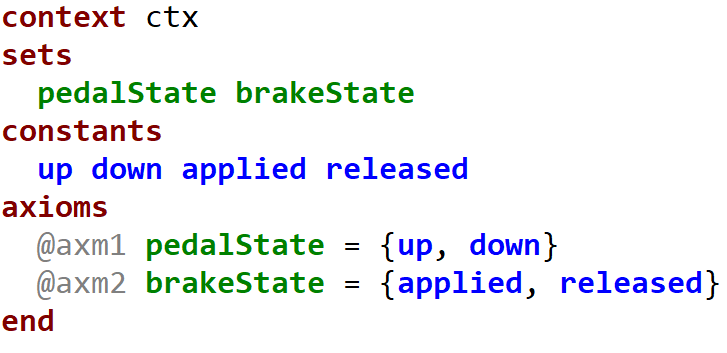
\includegraphics[scale = 0.3]{images/eventb4.PNG} }}
    \caption{Context of the brake example}
    \label{fig:brake1}
\end{figure}
\begin{figure}[h]
    \centering
    \subfloat{\frame{{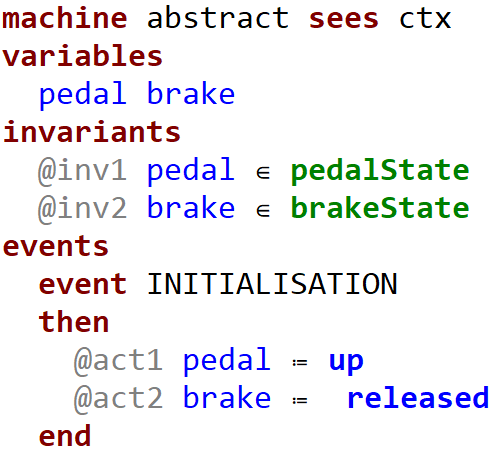
\includegraphics[scale = 0.3]{images/eventb5.PNG} }}}
    \quad
    \subfloat{\frame{{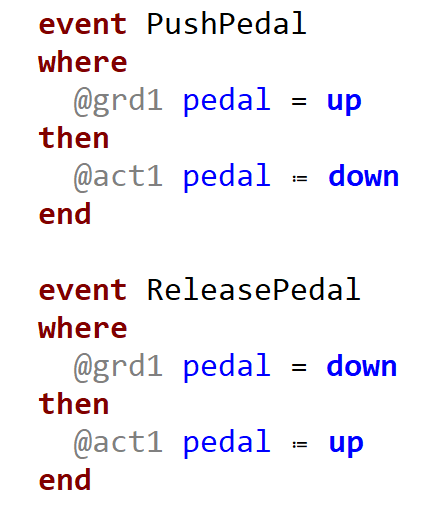
\includegraphics[scale = 0.3]{images/eventb6.PNG} }}}
    \quad
    \subfloat{\frame{{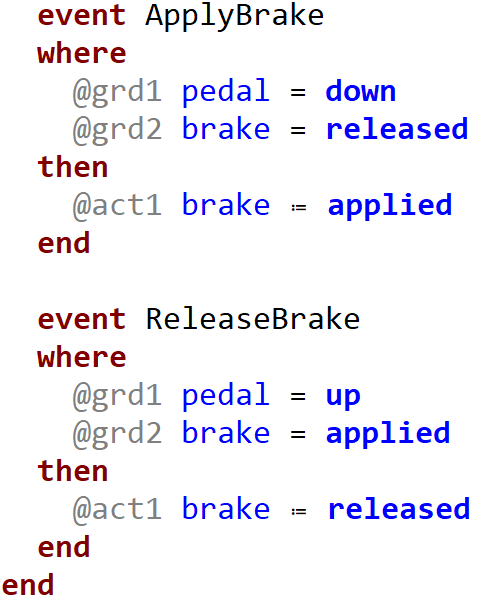
\includegraphics[scale = 0.3]{images/eventb7.PNG} }}}
    \caption{Machine of the brake example}
    \label{fig:brake2}
\end{figure}
The context identifier for this model is \textit{ctx}, the set of set identifiers is $\bar{s} = \{pedalState, brakeState\}$ and the set of constants is $\bar{c} = \{up, down, applied, released \}$. The $pedalState$ carrier set contains the possible states of the pedal ($up$ or $down$) and the $brakeState$ carrier set contains the possible states of the brake (applied or released). Both of these sets, are defined using the axioms $axm1 = A_1(\bar{s},\bar{c})$ and $axm2 = A_2(\bar{s},\bar{c})$. Therefore, the axioms of the brake model are defined by $A(\bar{s},\bar{c}) = A_1(\bar{s},\bar{c}) \land A_2(\bar{s},\bar{c})$. In particular, this context doesn't extend other components or uses theorems. 

For the model's machine, the machine identifier is \textit{abstract} and it "sees" the sets, constants and axioms in \textit{ctx}. The set of variables in the brake model is defined as $\bar{v} = \{pedal, brake\}$. The $pedal$ variable represents the pedal's state and the $brake$ variable represents the brake's state. Invariants $inv1 = I_1(\bar{v})$ and $inv2 = I_2(\bar{v})$ define the domain for variables $pedal$ and $brake$ respectively, by assigning to each one of them their respective carrier set. The resulting invariant for the brake model is $I(\bar{v}) = I_1(\bar{v}) \land I_2(\bar{v})$. Each one of the events in the model represent a state transition and a system action:
\begin{itemize}
    \item The \textit{INITIALISATION} event is executed when the model simulation starts. In this case, the action $S(\bar{t}, \bar{v})$ of the \textit{INITIALISATION} event is defined by the two assignments $pedal := up$ and $brake := released$.
     
    \item The \textit{PushPedal} event represents the action of pushing the pedal. The guard of the event $G(\bar{t}, \bar{v}) = G_1(\bar{t}, \bar{v}) = grd1$ states that he pedal must be \textit{up}, to execute the action $S(\bar{t}, \bar{v}) = S_1(\bar{t}, \bar{v}) = act1$. This action assigns the value \textit{down} to the \textit{pedal} variable. Conversely, the \textit{ReleasePedal} event guard verifies that the \textit{pedal} variable is \textit{down}, and changes its value to \textit{up} when executed.
    
    \item The \textit{ApplyBrake} event represents the action of applying the brake. The guard of the event $G(\bar{t}, \bar{v}) = G_1(\bar{t}, \bar{v}) \land G_2(\bar{t}, \bar{v}) = grd1 \land grd2$ states that the pedal must be \textit{down} and the brake \textit{released}, to execute the action $S(\bar{t}, \bar{v}) = S_1(\bar{t}, \bar{v}) = act1$. This action assigns the value \textit{applied} to the \textit{brake} variable. On the other hand, the \textit{ReleaseBrake} check for the opposite conditions ($pedal = up$ and $brake = applied$) and changes the value of the \textit{brake} variable to \textit{released}. 
\end{itemize}

\section{Non-deterministic choices in Event-B}
When an Event-B model is simulated or verified, there exists the possibility that in a system state there are multiple transition possibilities with multiple parameters that suffice all the model constraints. The way Event-B resolves this multiple choice dilemma is with \textit{non-deterministic choice} and there are 3 types of it:
\begin{itemize}
    \item \textbf{Choice of enabled events:} When multiple events are enabled for execution, i.e. when multiple events satisfy their event guards, one of them is chosen non-deterministically.  
    \item \textbf{Choice of parameter values:} In an event with parameters, it is possible to have multiple valuations for parameters $\bar{t}$ such that the guard of the event $G_i(\bar{t}, \bar{v})$ is satisfied. Therefore, the parameter that will be used in the execution of the event is chosen non-deterministically
    \item \textbf{Non-Deterministic assignments:} As mentioned before, there are 3 types of event assignments: deterministic assignment, predicate assignment and enumerated assignment. Both predicate and enumerated assignments, are non-deterministic for the following reason:
    \begin{itemize}
        \item Predicate assignment $x :\! | \; Q(\bar{t}, \bar{v}, x, x')$: means that the variable $x$ is assigned the value $x'$ that satisfies the predicate $Q(\bar{t}, \bar{v}, x, x')$. When there are multiple $x'$ values that satisfy the predicate, then the new value of $x$ is chosen non-deterministically.
        \item Enumerated assignment $x :\in  \{ E_1(\bar{t},\bar{v})... E_n(\bar{t},\bar{v}) \}$: states that to the variable $x$, one of the multiple expressions $E_i(\bar{t},\bar{v})$ in the set is assigned to it. This choice of which expression will be chosen, is done non-deterministically. 
    \end{itemize}
\end{itemize}
  


\section{Probabilistic Event-B}
Based on the 3 types of non-determinism present in Event-B, probabilistic Event-B \cite{Aouadhi2017} introduces probabilistic choices to replace non-deterministic ones in the following way:
\begin{itemize}
    \item \textbf{Probabilistic choice of enabled events:} To solve the non-determinisim, an expression $W_i(\bar{v})$ over the variables represents the \textit{weight} of a specific event $e_i$. Therefore, when multiple events are enabled, the probability of choosing one of them will be the ratio of its weight over the sum of all the weights of enabled events. This means that if there are $n$ events, then the probability of choosing event $e_i$ is $P(e_i) = \frac{W(e_i)}{\sum^{n}_{j = 1}W(e_j)}$
    \item \textbf{Probabilistic choice of parameter values:} In order to choose a parameter value probabilistically, a discrete uniform distribution can be used as a default choice to assign probabilities to the parameters. For that reason, the probability of choosing a parameter valuation $P(t_i) = \frac{1}{n}$ where $n$ is the number of parameter valuations that satisfy the guard of the event.
    \item \textbf{Predicate probabilistic assignment:} A predicate probabilistic assignment written as $x:\! \oplus \; Q(\bar{t}, \bar{v}, x, x')$ chooses the new value of $x$ with a uniform distribution. Hence, the probability of choosing a variable value $x'_i$ is $P(x'_i) = \frac{1}{n}$ where $n$ is the number of variable valuations that satisfy the predicate $Q(\bar{t}, \bar{v}, x, x')$. This probabilistic assignment replaces the non-deterministic predicate assignment. 
    \item \textbf{Enumerated probabilistic assignment:} A enumerated probabilistic assignment written as $x := E_1(\bar{t},\bar{v})@_{p_1}\oplus...\oplus E_n(\bar{t},\bar{v})@_{p_n}$  assigns a specific probability $p_i$ to each expression $E_i$, where $0 < p_i \leq 1$ and $p_1 + ... + p_n = 1$. This probabilistic assignment replaces the non-deterministic enumerated assignment.
\end{itemize}
Based on this changes, the new structure for probabilistic events can be defined as:
\begin{align*}
    e \; \equalhat \; \textbf{weight} \; W( \bar{v}) \; \textbf{any} \; \bar{t} \; \textbf{where} \; G(\bar{t}, \bar{v}) \; \textbf{then} \; S(\bar{t}, \bar{v}) \; \textbf{end} 
\end{align*}
Where $W( \bar{v})$ is an expression over the variables that determines the weight of the event, $\bar{t}$ is the set of parameters of the event, $G(\bar{t}, \bar{v})$ the guard of the event and $S(\bar{t}, \bar{v})$ is the \textit{probabilistic action}. The probabilistic action contains only deterministic assignments, predicate probabilistic assignments and enumerated probabilistic assignments. The resulting Machine for a probabilistic model is then $\mathscr{M} =(\bar{v}, I(\bar{v}), V(\bar{v}), PEvts, Init)$ where $PEvts$ is a set of probabilistic events and $Init \in PEvts$. To exemplify probabilistic Event-B, let's consider an extension of the previously explained brake model. This new example, presented also in \cite{Aouadhi2017}, adds new constraints:
\begin{itemize}
    \itema Pedal failure: when the driver tries to switch “down” the pedal, it may stay in the same position.
    \itemb Risk of pedal failure: the risk of pedal failure is set to 10\%.
    \itemc brake failure: the brake may not be applied, although the pedal has been switched down.
    \itemd Maximum brake wear: the brake cannot be applied more than a fixed number of times.
    \iteme Brake wear: due to brake wear, the risk of brake failure increases each time the brake is applied.
\end{itemize}
The resulting probabilistic model is displayed in figure \ref{fig:brake3}. This new model incorporates all of the previously defined constraints in the following way:
\begin{itemize}
    \item Constraints \textbf{R1} and \textbf{R2} are modeled in the probabilistic event \textit{PushPedal}, in which an enumerated probabilistic assignment is used to assign the value of variable \textit{pedal}. This assignment $pedal := down \ @9/10  \ \oplus \ up \ @1/10$ states that when the event \textit{PushPedal} is executed, the probability of changing its value to \textit{down} is $90\%$ and the probability of remaining with the value \textit{up} is $10\%$.
    \item For \textbf{R4}, a new constant \textit{MAX\_WEAR} $\in \mathbb{N}$ and \textit{MAX\_WEAR} $> 1$, is introduced to the context of the model. This constant determines the maximum number of times the break can be applied. In addition, the variable \textit{wear} $\in \mathbb{N}$ tracks the number of times the brake has been used. To make sure that the number of times the break has been applied doesn't exceeds the maximum wear, i.e. \textit{wear} $<$ \textit{MAX\_WEAR}, the weights of probabilistic events \textit{ApplyBrake} and \textit{ReleaseBrake} are modeled by the expression \textit{MAX\_WEAR} $-$ \textit{wear}. Therefore, when \textit{MAX\_WEAR} $=$ \textit{wear}, the weight of both events will be 0. This will make their probability of execution also 0, based on how probabilistic choice of enabled events is calculated.
    \item To model \textbf{R3}, a new event \textit{ApplyBrakeFailure} is introduced. When executed, this event simulates brake failure, by leaving the brake in state \textit{released}, when the pedal is \textit{down}.
    \item Finally, the constraint \textbf{R5} is defined by the weights of event \textit{ApplyBrake} and \textit{ApplyBrakeFailure}. As mentioned before, the weight of event \textit{ApplyBrake} is modeled with the expression \textit{MAX\_WEAR} $-$ \textit{wear}, and the expression for the weight of event \textit{ApplyBrakeFailure} is \textit{wear}. Thus, when the value of variable \textit{wear} increases, then the probability of executing event \textit{ApplyBrake} decreases and the probability of \textit{ApplyBrakeFailure} increases. 
    
    \end{itemize}
\begin{figure}[h]
    \centering
    \subfloat{\frame{{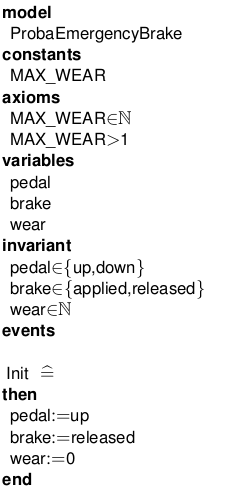
\includegraphics[scale = 0.3]{images/eventb8.PNG} }}}
    \quad
    \subfloat{\frame{{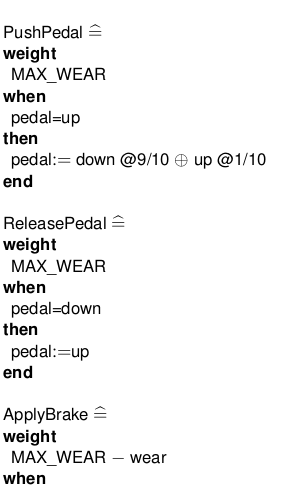
\includegraphics[scale = 0.3]{images/eventb9.PNG} }}}
    \quad
    \subfloat{\frame{{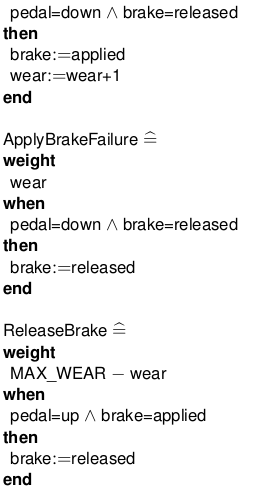
\includegraphics[scale = 0.3]{images/eventb10.png} }}}
    \caption{Probabilistic machine of the brake example, taken from \cite{Aouadhi2017}}
    \label{fig:brake3}
\end{figure}




\section{Maude}
%Main sources for this chapter: PeterMaude, Lecture1, Lecture3

%explain the generality of Maude
Maude \cite{MaudeManual, PeterMaude, Lecture1} is a high performance declarative language, that allows the specification of programs or systems, and their formal verification.
%explain how Maude program are written in functional module (sorts, subsorts, ops, etc, equations and equation evaluation)
Maude's programs are represented as \textit{functional modules} declared with syntax:
\begin{lstlisting}
fmod MODULENAME is
    BODY
endfm
\end{lstlisting}
where \textit{MODULENAME} is the name of the functional module, and \textit{BODY} is a set of declarations that specify the program. The body of the module contains \textit{sorts} (written in Maude as \texttt{sorts}), where each sort correspond to a specific data type of the program. It also contains a set of function symbols or function declarations called \textit{operators} (abbreviated as \texttt{op} in Maude), that specify the constructors of the different sorts, along with the syntax of the program functions. Finally, a set of \textit{equations} (abbreviated as \texttt{eq} in Maude) is used to define the behavior of the functions. These equations use \textit{variables} (abbreviated as \texttt{var} in Maude) to describe how each function works. 

%provide an example of a maude program functional module
To illustrate how a Maude program is contructed, the following code corresponds to a program that defines the natural numbers and the addition operation, borrowed from \cite{PeterMaude}: 
\begin{lstlisting}
fmod NAT-ADD is
  sort Nat .

  op 0 : -> Nat [ctor] .
  op s : Nat -> Nat [ctor] .
  op _+_ : Nat Nat -> Nat .

  vars N M : Nat .
    
  *** Recursive Definition for addition
  eq N + 0 = N .
  eq N + s(M) = s(N + M) .
endfm
\end{lstlisting}
The sort \texttt{Nat} is a data type that represents the natural numbers. This sort has two constructors (represented in the code with the key word \texttt{ctor}): 0 which is a constant and the operator \texttt{s}, which takes one argument of type \texttt{Nat} and represents the successor function in the natural numbers. With these two operators, it is possible to define arithmetic functions in the natural numbers, like addition or multiplication. In this module, both functions are defined inductively using equations. Using this module, it is possible to compute the value for addition or multiplication for two natural numbers using the command \texttt{red}. For example, if the command \texttt{red s(s(s(0))) + s(s(0))} is used, that represents the operation 3 + 2, the answer 5 is obtained represented as \texttt{s(s(s(s(s(0)))))}:
\begin{lstlisting}
*********** equation
eq N + s(M) = s(N + M) .
N --> s(s(s(0)))
M --> s(0)
s(s(s(0))) + s(s(0))
--->
s(s(s(s(0))) + s(0))
*********** equation
eq N + s(M) = s(N + M) .
N --> s(s(s(0)))
M --> 0
s(s(s(0))) + s(0)
--->
s(s(s(s(0))) + 0)
*********** equation
eq N + 0 = N .
N --> s(s(s(0)))
s(s(s(0))) + 0
--->
s(s(s(0)))
result Nat: s(s(s(s(s(0)))))
\end{lstlisting}
Maude computes using equations from left to right. Therefore, in computation steps like the first one, the expression \texttt{s(s(s(0))) + s(s(0))} is matched with the left side of the equation \texttt{N + s(M) = s(N + M)} and matching substitution $\{\texttt{N} \mapsto \texttt{s(s(s(0)))},\texttt{M} \mapsto \texttt{s(0)} \}$. The resulting expression \texttt{s(s(s(0))) + s(s(0))}, will be simplified again with the same equation, until it reduces to a simplified expression that can be matched with the equation \texttt{N + 0 = N} (as seen in the last step).

%explain the semantics behind the functional modules
Semantically, functional modules in Maude are represented as \textit{equational theories} \cite{Lecture1,PeterMaude}, that are represented as a pair $(\Sigma, E)$ where: 
\begin{itemize}
    \item the \textit{signature} $\Sigma$ describes the syntax of the theory, which is the data types and operators symbols (sorts and operators).
    \item $E$ is the set of equations between expressions written in the syntax of $\Sigma$.
\end{itemize}
As mentioned before, computations in Maude are done by using the equations over expressions constructed with operators. This method is called \textit{term rewriting} \cite{Lecture1,PeterMaude} and behaves in the following way: 

\begin{itemize}
    \item With the equations $E$ of $(\Sigma, E)$, \textit{term rewriting rules} are defined as $\vv{E} = \{u \rightarrow v  \ | \ (u = v) \in E \}$. 
    \item A term $t$, which are expressions formed using the syntax in $\Sigma$, is rewritten to $t'$ in one step $t \rightarrow_{\vv{E}} t'$ if and only if, the following conditions are sufficed:
        \begin{itemize}
            \item there is a subterm $w$ in $t$, expressed as $t[w]$.
            \item there is a rule $(u \rightarrow v) \in \vv{E}$ and a substitution $\theta$ s.t. : $w = u\theta$, $w' = v\theta$, $t'=t[w']=t[v\theta]$.   
        \end{itemize}
\end{itemize}
for example, in the previous computation \texttt{red s(s(s(0))) + s(s(0))} the term rewriting process in the second step, is the following:
\begin{itemize}
    \item $E = \texttt{N+s(M)=s(N + M)}$
    \item $t = \texttt{s(s(s(s(0))) + s(0))}$
    \item $\theta = \{\texttt{N} \mapsto \texttt{s(s(s(0)))},\texttt{M} \mapsto \texttt{0} \}$
    \item $w = \texttt{N+s(M)}\theta = \texttt{s(s(s(0))) + s(0)}$
    \item $w' = \texttt{s(N+M)}\theta = \texttt{s(s(s(s(0))) + 0)}$
    \item $t' = \texttt{s}([w']) = \texttt{s(s(s(s(s(0))) + 0))}$
\end{itemize}
the resulting term rewriting is $t \rightarrow_{\vv{E}} t'$.
%explain the functional modules with rewriting rules
%explain theory behind it
Aside from building programs in Maude using functional modules, it is also possible to model concurrent systems. This is done with \textit{system modules}, which permits the construction of system states and transitions. Semantically, a system module is a \textit{rewrite theory} \cite{PeterMaude,Lecture3} $\mathscr{R} = (\Sigma, E, L, R)$ where: 
\begin{itemize}
    \item $(\Sigma, E)$ is an equational theory.
    \item $L$ is a set of labels.
    \item $R$ is a set of unconditional labeled rewrite rules of the form $l: t \rightarrow t'$, and conditional labeled rewrite rules of the form $l: t \rightarrow t' \ \text{if} \ cond$, where $l \in L$, $t,t'$ are terms in $\Sigma$ and $cond$ is a condition or system guard.    
\end{itemize}
The syntax for system modules in Maude is:
\begin{lstlisting}
mod MODULENAME is
    BODY
endm
\end{lstlisting}
Where the body represents a rewrite theory $\mathscr{R}$. The syntax for unconditional rewriting rules is
\begin{lstlisting}[mathescape=true]
rl [$l$] : $t$ => $t'$ .
\end{lstlisting}
and for conditional rewriting rules is
\begin{lstlisting}[mathescape=true]
crl [$l$] : $t$ => $t'$ if $cond$ .
\end{lstlisting}
%provide an example of a model
to exemplify this, let's consider the following simple model of a bus: A transport bus has capacity for 60 people. The bus can be moving or stationary, and can only drop or lift passengers when the bus is stationary. Finally, at any time the bus driver can use the brake to stop or use the gas pedal to move. The corresponding Maude system module for this model is:
\begin{lstlisting}
mod BUS is protecting NAT .
  sorts Bus Status .

  op bus : Nat Status -> Bus [ctor] .
  ops stationary moving : -> Status [ctor] .
 
  vars N M : Nat . var S : Status .

  *** move the bus
  rl [move] : bus(N,stationary) => bus(N,moving) .
  *** stop the bus 
  rl [stop] : bus(N,moving) => bus(N,stationary) .
  *** drop passenger
  rl [drop] : bus(s(N),stationary) => bus(N,stationary) .
  *** lift passenger
  crl [lift] : bus(N,stationary) => bus(s(N),stationary) 
                                    if s(N) <= 60 . 
endm
\end{lstlisting}
%explain how the maude model corresponds to the theory
In this model the states of the system are represented with instances of the sort \texttt{Bus}, and it contains a natural number that represents the number of people inside the bus and a \texttt{Status}, which represents the state of the bus (it can be stationary or moving). In this case, no equations are used, therefore the set of equations $E = \emptyset$  and $\Sigma$ will contain the sorts \texttt{Bus} and \texttt{Status} with their respective operators. To model the different events in the model, 4 rewriting rules were used:
\begin{itemize}
    \item An unconditional rule, labeled \texttt{move}, that represents the event of using the gas pedal to move the bus by changing the status from \texttt{stationary} to \texttt{moving}. Note that this rule can only be applied when the bus is \texttt{stationary}, as stated by the rule first term \texttt{bus(N,stationary)}.
    \item An unconditional rule, labeled \texttt{stop}, that represents the event of using the brakes to stop the bus. This changes the status of the bus from \texttt{moving} to \texttt{stationary}. As the previous rule, it can only be applied when the first term is matched, i.e. when the bus status is \texttt{moving}. 
    \item An unconditional rule, labeled \texttt{drop}, that represents the event of dropping people off the bus. The subterm \texttt{s(N)} assures that it can only drop a person when the number of people in one or more. This rule rewrites the state of the system, by reducing the number of passengers in the bus by one.
    \item A conditional rule, labeled \texttt{lift}, that represents the event of lifting a passenger. When this rules are applied, the number of passengers inside the bus is increased by one. To prevent exceeding the maximum capacity of the bus, the condition \texttt{if s(N) <= 60} is used. 
\end{itemize}
With this system module, that represents a rewrite theory $\mathscr{R}$, the simple bus model can be specified and verified using other functionalities in Maude like model checking with the commands \texttt{rewrite} and \texttt{search}. The \texttt{rewrite} command or \texttt{rew} takes an initial state of the system and uses the rewriting rules until termination, i.e. until no other rewriting rule can be applied to the system state. In the case of the bus example, the rules \texttt{move} and \texttt{stop} can be applied infinitely. Therefore, to be able to simulate this system, Maude also allows to use bounded rewriting. With this method, it is possible to specify the number of rewriting rules to be applied to the initial state of the system. For example, the command \texttt{rew [3] bus(0, stationary) .} will apply 3 rewriting rules to the state \texttt{bus(0, stationary)}, which refers to a stationary bus with no passengers. The resulting execution is:
\begin{lstlisting}
*********** rule
rl bus(N, stationary) => bus(N, moving) [label move] .

bus(0, stationary)
--->
bus(0, moving)
*********** rule
rl bus(N, moving) => bus(N, stationary) [label stop] .

bus(0, moving)
--->
bus(0, stationary)
*********** rule
crl bus(N, stationary) => bus(s N, stationary) if s N <= 60 = true [label lift] .

bus(0, stationary)
--->
bus(1, stationary)
result Bus: bus(1, stationary)
\end{lstlisting}
Lastly, with the \texttt{search} command it is possible to verify if a given state is reachable. For example, to check if the state \texttt{bus(10,stationary)} can be reached from the initial state \texttt{bus(0,moving)}, the command \texttt{search bus(0,stationary) =>* bus(10, moving) .}  can be used. The result of this command is:
\begin{lstlisting}
search in BUS : bus(0, stationary) =>* bus(10, moving) .

Solution 1 (state 21)
states: 22  rewrites: 50 in 0ms cpu (0ms real) (~ rewrites/second)
empty substitution

No more solutions.
\end{lstlisting}
If the search returns a solution, it means that the state is reachable. Furthermore, it is also possible to check if the system will exceed the maximum capacity, defining a system invariant $I$ that states this property. This can be done, by adding the following code to the bus module:
\begin{lstlisting}
*** Define predicates
  var X : Bus .
  op predicate : Bus -> Bool .
  eq predicate(bus(N,S)) = if N <= 60 then true else false fi .
\end{lstlisting}
This invariant can be checked with the \texttt{search} command using:
\begin{lstlisting}
search bus(0,stationary) =>* X  s.t. predicate(X) =/= true .
\end{lstlisting}
which searches for a state \texttt{X} where the bus has more than 60 passengers. The resulting execution of the command returns no solution:
\begin{lstlisting}
search in BUS : bus(0, stationary) =>* X such that predicate(X) =/= true = true .

No solution.
\end{lstlisting}
This means that the bus system can not exceed the maximum capacity of the bus.
\section{Object-Based Programming in Maude}
Object-based programming in Maude \cite{MaudeManual, Lecture3, PeterMaude} is supported by a predefined module \texttt{CONFIGURATION}. This module contains the necessary sorts and syntax to define the objects, messages, system configurations and objects interactions, of an object-based system. This module is defined as:
\begin{lstlisting}
mod CONFIGURATION is
  *** basic object system sorts
  sorts Object Msg Configuration .
  *** construction of configurations
  subsort Object Msg < Configuration .
  op none : -> Configuration [ctor] .
  op __ : Configuration Configuration -> Configuration
[ctor config assoc comm id: none] .
\end{lstlisting}

The basic sorts are \texttt{Object}, \texttt{Msg} and \texttt{Configuration}. A term of sort \texttt{Object} represents an instance of a system object, a term of sort \texttt{Msg} represents a message shared by the system objects and a term of sort \texttt{Configuration} represents a snapshot of the current system state, represented as a multiset of objects and messages. These configurations are built with the multiset union operation (defined with syntax \texttt{\_\,\_} ) between objects, messages or other configurations, and the empty configuration is defined as \texttt{none}. The module configuration also implements a predefined syntax for object construction. They have the form:
\begin{align*}
    \langle O : C \ | \ a_1:v_1,...a_n:v_n \rangle
\end{align*}
Where $O$ is the object's identifier, $C$ is its class, $a_1...a_n$ are attribute identifiers and $v_1...v_n$ are the values of each one of the attributes. This defined syntax in Maude is implemented as:
\begin{lstlisting}
  *** Maude object syntax
  sorts Oid Cid .
  sorts Attribute AttributeSet .
  subsort Attribute < AttributeSet .
  op none : -> AttributeSet [ctor] .
  op _,_ : AttributeSet AttributeSet -> AttributeSet
  [ctor assoc comm id: none] .
  op <_:_|_> : Oid Cid AttributeSet -> Object [ctor object] .
endm
\end{lstlisting}
Where \texttt{Oid} corresponds to the object identifier $O$, \texttt{Cid} is the class identifier $C$ and the attributes of the object are represented as a multiset. Messages' syntax is defined by the user. To understand how systems are modeled in Maude with configurations, the bank account example in \cite{MaudeManual} can be examined:
%provide an example
\begin{lstlisting}
mod BANK-ACCOUNT is
    protecting INT .
    protecting CONFIGURATION .
    op Account : -> Cid [ctor] .
    op bal :_ : Int -> Attribute [ctor gather (&)] .
    op from_to_transfer_ : Oid Oid Nat -> Msg [ctor] .
    
    vars A B : Oid .
    vars M N L : Nat .

    *** Definition of transfer rewriting rule
    crl [transfer] :
      (from A to B transfer M)
      < A : Account | bal : N >
      < B : Account | bal : L >
      => < A : Account | bal : N - M >
         < B : Account | bal : L + M >
      if N >= M .

    *** Definition of the initial configuration
    op bankConf : -> Configuration .
    ops A-001 A-002 : -> Oid .
    eq bankConf
    = < A-001 : Account | bal : 250 >
      < A-002 : Account | bal : 1250 >
      (from A-002 to A-001 transfer 300) .
endm
\end{lstlisting}
The system consists of different bank accounts, that can transfer money to each other. The bank account class is named as \texttt{Account}, and it contains the attribute \texttt{bal} which corresponds to the amount of money available in an account. The message \texttt{from\_to\_transfer\_} simulates the transfer request from one account to another, by specifying the two account object identifiers or Oid (one for the account that sends the money and the other one for the account that receives the money) and the amount of money to be sent as an integer. The rewrite rule \texttt{transfer} matches a system configuration where the message \texttt{from A to B transfer M} and the two accounts with Oid \texttt{A} and \texttt{B} are present. After that, the rule modifies the attribute \texttt{bal} of both accounts according to the transaction parameters and erases the message from the configuration. For example, if the initial configuration of the system is the one defined by \texttt{bankConf}, the result after using the rewriting command \texttt{rew in BANK-ACCOUNT : bankConf .} would be:
\begin{lstlisting}
result Configuration: < A-001 : Account | bal : 550 > 
                      < A-002 : Account | bal : 950 >
\end{lstlisting}

\section{PMaude}
%acknowledge the PMaude paper
%explain what PMaude is (probably use the thesis proposal)
Probabilistic Maude or PMaude \cite{Agha2006}, is a Maude extension that introduces probabilities to the language. The underlying theory behind PMaude are  \textit{probabilistic rewrite theories} which correspond to an extension of rewrite theories: probabilistic rewrite theories can be expressed as tuple $\mathscr{R}_p = (\Sigma, E, L, R, \pi)$, where $(\Sigma, E, L, R,)$ is a rewrite theory and $\pi$ is a function that assigns to each rewrite rule $r \in R$ a probability, given the current model state or configuration. This probability will determine if a rule may or may not be executed in the following system transition. The general form of probabilistic rewrite rules, for unconditional and conditional respectively is:
\begin{align*}
    l &: t(\overrightarrow{x}) \rightarrow t'(\overrightarrow{x}, \overrightarrow{y}) \; \text{if} \; C(\overrightarrow{x}) \; \textbf{with probability} \; \overrightarrow{y} := \pi_r(\overrightarrow{y}) \\
    l' &: t(\overrightarrow{x}) \rightarrow t'(\overrightarrow{x}, \overrightarrow{y}) \; \textbf{with probability} \; \overrightarrow{y} := \pi_r(\overrightarrow{y})  
\end{align*}
Where $\overrightarrow{x}$ is the set of variables of the current model state,  $\overrightarrow{y}$ is the set of new variables accessible in the following model state and $C(\overrightarrow{x})$ is the conjunction of conditions over the set $\overrightarrow{x}$. Moreover, $l, l'$ are labels in $L$, $t,t'$ are terms written with $\Sigma$ and $\pi_r$ corresponds to the probability function assigned to the specific rule $r \in R$. 
%provide the clock example and explain it
Let's consider the PMaude module, presented in \cite{Agha2006}: 
\begin{lstlisting}[mathescape=true]
pmod EXPONENTIAL-CLOCK is
  *** the following imports positive real number module
  protecting POSREAL .

  *** the following imports PMaude module that defines 
  *** the distributions EXPONENTIAL, BERNOULLI, GAMMA, etc.
  protecting PMAUDE .

  *** declare a sort Clock
  sort Clock .
  *** declare a constructor operator for Clock
  op clock : PosReal PosReal => Clock .
  *** declares a constructor operator for a broken clock
  op broken : PosReal PosReal => Clock .

  *** T is used to represent time of clock,
  *** C represents charge in the clocks battery,
  *** t represents time increment of the clock
  vars T C t : PosReal . var B : Bool .
  
  rl [advance]: clock(T,C) =>
                      if B then
                           clock(T+t,C - $\frac{\text{C}}{1000}$)
                      else
                           broken(T,C - $\frac{\text{C}}{1000}$)
                      fi
                with probability B:=BERNOULLI($\frac{\text{C}}{1000}$) 
                                and 
                                t:=EXPONENTIAL(1.0).
                
  rl [reset]: clock(T,C) => clock(0.0,C) .
endpm
\end{lstlisting}
This model represents a clock that works with a battery. The idea is to model the behavior of the clock, when the battery starts depleting: when the charge of the battery is high, then the probability that the clock breaks is low. Conversely, when the clock's battery is low, the clock has a higher probability of breaking. In this probabilistic system module, the clock is represented as a term \texttt{clock(T,C)}, where \texttt{T} is the time and \texttt{C} is the charge of the clock. The main probabilistic rewrite rule \texttt{advance} represents the "ticks" of the clock. If the boolean value \texttt{B} is true, then the clocks ticks normally and the new time will be the current time \texttt{T} plus an increment \texttt{t}. Also, the charge of the clock will be reduced by a thousandth of the current's clock's charge. If \texttt{B} is false, then the clock will break and change to the state \texttt{broken(T,C - $\frac{\texttt{C}}{1000}$)}. The constructor \texttt{broken} of sort \texttt{Clock}, represents the broken state of the clock. To incorporate the probabilistic choice of event for the clock's state (either ticking or breaking), the value \texttt{B} is chosen probabilistically, based on the charge of the clock. This is done by the \texttt{BERNOULLI} function, which receives a float number and returns a boolean value that is distributed according to the Bernoulli distribution with mean $\frac{\texttt{C}}{1000}$. Therefore, the lesser the charge left in the battery, the greater is the probability that the clock will break. The value \texttt{t} is also probabilistically determined, in this case, by an exponential distribution function.
There is also a second rewriting rule, that resets the clock to its initial state \texttt{clock(0.0, C)}. It is important to remark that this model has both probabilistic and non-deterministic choice: The state of the clock depends on a probability function but the choice of rewriting rules is done non-dereministically by Maude's fair scheduler.

PMaude modules can be transformed into regular system modules in Maude. This is done with three key modules: \texttt{COUNTER}, \texttt{RANDOM} and \texttt{SAMPLER}. The built-in \texttt{COUNTER} module in Maude consists of the rewriting rule
\begin{lstlisting}
rl counter => N:Nat .
\end{lstlisting}
that rewrites the constant counter to a natural number. The module is built to guarantee that every time the constant counter is replaced with a natural number \texttt{N}, this natural number corresponds to the successor of the natural number obtained in the previous use of the rule. The built-in \texttt{RANDOM} module provides a random number generator function, called \texttt{random}. Lastly, the \texttt{SAMPLER} module specifies the sampling functions for different probability functions. For example, for the previous clock example, the needed functions will be:
\begin{lstlisting}
op EXPONENTIAL : PosReal => PosReal .
op BERNOULLI : PosReal => Bool .
\end{lstlisting}
that are defined as:
\begin{lstlisting}
rl EXPONENTIAL(R) => (- log(rand)) / R .
rl BERNOULLI(R) => if rand < R then true else false fi .
\end{lstlisting}
The value \texttt{rand} in both of the rules is defined as:
\begin{lstlisting}
rl [rnd] : rand => float(random(counter + 1) / 4294967296) .
\end{lstlisting}
and it is rewritten in each step to a random number between 0 and 1. The number 4294967296 is used to divide the number returned by \texttt{random}, since it is the maximum number the function can return. The resulting Maude system module \cite{Agha2006} is:
\begin{lstlisting}[mathescape=true]
mod EXPONENTIAL-CLOCK-TRANSFORMED is 
  *** The SAMPLER mode includes the COUNTER and RANDOM modules
  protecting SAMPLER .
  protecting POSREAL .
  
  sort Clock . 
  op clock : Nat Float -> Clock [ctor] . 
  op broken : Nat Float -> Clock [ctor] . 
  
  vars T C : PosReal . 
  
  rl clock(T,C) => if BERNOULLI($\frac{\text{C}}{1000}$) then 
                        clock(T + EXPONENTIAL(1.0), C - $\frac{\text{C}}{1000}$) 
                   else 
                        broken(T,C - $\frac{\text{C}}{1000}$)
                   fi .
  
  rl [reset]: clock(T,C) => clock(0.0,C) .
endm
\end{lstlisting}

\section{VeStA, PVeStA, MultiVeStA and QuaTEx}
%explain what is VeStA
VeStA \cite{Vesta} is a tool (implemented in Java) for statistical analysis of probabilistic systems. It supports statistical model checking and statistical evaluation of expected values of temporal expressions. These expressions can be constructed using the query language of  \textit{Quantitative Temporal Expression} or QuaTEx \cite{Agha2006}, and analyzed by VeStA using \textit{Monte Carlo simulations} . 
%explain how VeStA works
The general process to use VeStA and analyze the properties of a probabilistic model, is the following:
\begin{enumerate}
    \item Create a probabilistic system in the supported modeling languages, e.g. probabilistic rewrite theories specified in PMaude.
    \item Define the model properties that are going to be analyzed using the supported temporal expressions, e.g. QuaTEx.
    \item Run Monte Carlos simulations using VeStA, over the model and the defined properties, specifying the simulation parameters.
    \item Get the expected value of the temporal expressions specified in step 2.
\end{enumerate}
%explain how Quatex works
The syntax of a QuaTEx expression is defined in figure \ref{fig:multivesta}. The reader can find an in depth explanation of this syntax and how QuaTEx queries evaluate in \cite{Agha2006,multivesta}, but for now we will define a QuaTEx expression as the expected value of a temporal logic predicate over state observations (i.e. the value of the variables of a model in a given configuration) that returns a real number (i.e. a \textit{real-typed predicate}). For example the QuaTEx expression \texttt{eval E[$PExp$]} returns the expected value of the real number returned by the temporal logic predicate $PExp$ (or also called \textit{path expression} in the syntax of QuaTEx).  
\begin{figure}[h]
    \centering
    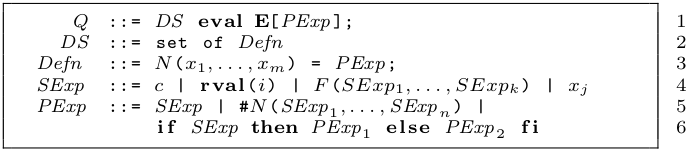
\includegraphics[scale = 0.4]{images/quatex1.png}
    \caption{QuaTEx syntax, taken from \cite{multivesta}}
    \label{fig:multivesta}
\end{figure}

Using the previous definition of QuaTEx queries, let's suppose that we want to find the expected value of a QuaTEx query \texttt{eval E[$PExp$]} using VeStA (we will refer to the expected value of the QuaTEx query obtained by VeStA as $\bar{x}$, and to the real expected value as $x$). To obtain $\bar{x}$, VeStA uses 2 user-defined parameters $\alpha$ and $\delta$. With these parameters, VeStA runs $n$ simulations, until $n$ is large enough to obtain a \textit{confidence interval} (CI) with probability $(1-\alpha) * 100\%$ bounded by $\delta$, i.e an interval $[\bar{x} - \frac{\delta}{2},\bar{x} + \frac{\delta}{2}]$ where the probability that $x \in [\bar{x} - \frac{\delta}{2},\bar{x} + \frac{\delta}{2}]$ is $(1-\alpha) * 100\%$. In other words, if VeStA calculates the expected value of a QuaTEx query as $\bar{x}$, then the probability that the real expected value of the query (represented as $x$) is in the interval $[\bar{x} - \frac{\delta}{2},\bar{x} + \frac{\delta}{2}]$, is $(1-\alpha) * 100\%$ (An example will be presented in the next section to illustrate this)

Based on this, the authors in \cite{AlTurki2011} present an extension of VeStA called PVeStA. This tool allows to run parallelized algorithms for statistical model checking using a client-server architecture. Furthermore \cite{multivesta} presents an extension of both VeStA and PVeStA called MultiVeStA, that extends the QuaTEx language to MultiQuaTEx, by allowing to query more state measures at a time. This improves the usability and the performance of the language. The extension also integrates existing discrete event simulators in addition to the originally supported ones, and improves the presentation of results. In the following section, an explanation of the use of MultiVeStA will be given, to illustrate all the concepts explained in this section.

\section{Using MultiVeStA}
The aim of this section is to provide a simple tutorial on how to use the MultiVeStA tool, since the available information online is very limited. Generally speaking, the blueprint to modify and run any PMaude model to be used by MultiVeStA is:
\begin{enumerate}
    \item Define the PMaude model's states as configurations using object-oriented programming in Maude and define the system transitions as rewriting rules between configurations.
    \item Include the necessary elements of MultiVeStA inside the model's definition.
    \item Define an analysis module to define the model observations used by the QuaTEx queries.
    \item Define the QuaTEx queries that represent the model's properties that want to be checked.
    \item Specify the simulation parameters.
    \item Run the simulations using the the probabilistic model, the QuaTEx queries and the simulation parameters.
\end{enumerate}
We will walk-through this steps with a practical example, where we aim to verify properties over the PMaude model of the clock model presented in section 2.6. Before we start, it is important to mention that the version of the MultiVeStA tool used for this example can be found in \cite{multiTool}. In this GitHub page, the reader can find the instructions to download and run MultiVeStA. It is important that the reader runs the prepared \texttt{dice.maude} example and read the \texttt{README} file, to get to know the tool.
\subsection{Step 1: Object-based clock example}
First of all, we will start from the following specification of the clock model explained in section 2.6 (with file name \texttt{clock.maude}) taken from \cite{MaudeManual}:
\begin{lstlisting}
mod CLOCK is 
  pr SAMPLER . 
  sort Clock . 
  op clock : Nat Float -> Clock [ctor] . 
  op broken : Nat Float -> Clock [ctor] . 
  var T : Nat . 
  var C : Float . 
  rl clock(T,C) => if sampleBernoulli(C / 1000.0) 
     			   then clock(s(T), C - (C / 1000.0)) 
                   else broken(T, C) 
                   fi . 
endm
\end{lstlisting}
To transform this specification into an object oriented one, we will divide it in different modules. The first one is the module \texttt{SORTS}, where the different sorts of the attributes of the configuration or class will be specified. In this case, a sort \texttt{State} that has two constants \texttt{working} and \texttt{broken}:
\begin{lstlisting}
mod SORTS is
  sort State .
  op working : -> State [ctor] .
  op broken : -> State [ctor] .
endm
\end{lstlisting}
The second module is \texttt{ATTRIBUTES}, where the attributes , the class identifier and the object identifier of the model's states are defined:
\begin{lstlisting}
mod ATTRIBUTES is
  pr CONFIGURATION .
  pr NAT .
  pr FLOAT .
  pr SORTS .
  op Clock : -> Cid [ctor] .
  op myClock : -> Oid [ctor] .
  op time:_ : Nat -> Attribute [ctor] . 
  op battery:_ : Float -> Attribute [ctor] . 
  op state:_  : State -> Attribute [ctor] . 
endm
\end{lstlisting}
The third module is \texttt{SCENARIO} where the initial state of the system is going to be defined. It is important to mention, that the name of the initial state must be \texttt{init}, so MultiVeStA can recognize it:
\begin{lstlisting}
mod SCENARIO is
  pr ATTRIBUTES .
  op init : -> Configuration .
  eq init = < myClock : Clock  | time: 0, 
              battery: 1000.0, state: working > . 
endm
\end{lstlisting}
The fourth module, is the \texttt{DYNAMICS} module. This module will contain the conditional and unconditional rewriting rules of the model:
\begin{lstlisting}
mod DYNAMICS is
  pr SCENARIO .
  pr SAMPLER . *** Using the previously defined sampler
  var cl : Oid .
  var T : Nat .
  var C : Float .
  
  rl [clockTick] :
    < cl : Clock  | time: T, battery: C, state: working > 
  =>
    if sampleBernoulli(C / 1000.0) then
      < cl : Clock  | time: s(T), battery: (C - (C / 1000.0)), state: working >
    else
      < cl : Clock  | time: T, battery: C, state: broken >
    fi .
endm
\end{lstlisting}
The module \texttt{SAMPLER} is the same sampler module defined for the clock example in the PMaude section. If we include all this modules in the same file, named \texttt{clock.maude}, we can load the file to maude and apply the \texttt{rew} and \texttt{search} to verify and test the specification as one would normally do with other system modules. 

\subsection{Step 2: Including MultiVeStA elements}
First, in the \texttt{SORTS} module include the \texttt{APMAUDE} module that comes with the tool in the \texttt{apmaude.maude} file. The \texttt{APMAUDE} module includes other predefined Maude modules like \texttt{CONFIGURATION} (where the \texttt{Configuration} sort is renamed to \texttt{Config}), \texttt{NAT}, \texttt{FLOAT} and \texttt{STRING}. After that, for each one of the rewriting rules specified in \texttt{DYNAMICS}, create a constant, with the exact name of the label of the rule, of sort \texttt{Content} (The sort content is defined inside the \texttt{APMAUDE} module). The resulting \texttt{SORTS} module is:
\begin{lstlisting}
mod SORTS is
  pr APMAUDE .
  sort State .
  op working : -> State [ctor] .
  op broken : -> State [ctor] .
  op clockTick : -> Content [ctor] .
endm
\end{lstlisting}
Since the \texttt{APMAUDE} includes the sorts \texttt{CONFIGURATION}, \texttt{NAT}, \texttt{FLOAT}, then in the \texttt{ATTRIBUTES} module is no longer necessary to include again these modules, because they will be included in \texttt{SORTS}. In the \texttt{SCENARIO} module, the initial configuration of the system must be modified to:
\begin{lstlisting}
mod SCENARIO is
  pr ATTRIBUTES .
  op init : -> Configuration .
  eq init = {0.0 | [ 1.0 , (myClock <- clockTick),0] }
            randomCounter(0)
            < myClock : Clock  | time: 0, battery: 1000.0, state: working > . 
endm
\end{lstlisting}
In this new \texttt{init} configuration there are 3 objects:
\begin{itemize}
    \item The first one is a construction used by MultiVeStA, and states that the initial time is 0.0, the initial event or rule to be applied is \texttt{clockTick} (which corresponds to the constant of type \texttt{Content} specified in the \texttt{SORTS} module) and it would be applied at time 1.0 to the object with Oid \texttt{myClock}.
    \item The second object \texttt{randomCounter}is a counter used to generate pseudo-random numbers, and is initialized to 0. MultiVeStA also requires the definition of this object to run the simulations.
    \item The third object corresponds to the same initial state of the model presented in the previous \texttt{SCENARIO} module.
\end{itemize}
Finally, the module \texttt{DYNAMICS} must be modified to:
\begin{lstlisting}
mod DYNAMICS is
  pr SCENARIO .
  pr SAMPLER .

  *** variables used for Multivesta processes
  var gt : Float .  
  var SL : ScheduleList .
  var explCounter : Nat .

  *** state variables
  var cl : Oid .
  var T : Nat .
  var C : Float .


  crl [clockTick] :
    { gt | SL } (cl <- clockTick)
    { < cl : Clock  | time: T, battery: C, state: working > 
      randomCounter(explCounter) }
  =>
    if sampleBernoulli(explCounter, (C / 1000.0)) then
      insert({ gt | SL },[ gt + 1.0 , (cl <- clockTick),0])
      { < cl : Clock  | time: s(T), 
                        battery: (C - (C / 1000.0)), state: working > 
        randomCounter(s(explCounter)) }
    else
      insert({ gt | SL },[ gt + 1.0 , (cl <- clockTick),0])
      { < cl : Clock  | time: T, battery: C, state: broken > 
        randomCounter(s(explCounter)) }
    fi .

endm
\end{lstlisting}
This new module includes the following changes:
\begin{itemize}
    \item The protected \texttt{SAMPLER} module corresponds to the sampler defined in the \texttt{apmaude.maude} file. This new sampler uses a counter to generate random number. That is why the new call of the function \texttt{sampleBernoulli} has an additional parameter \texttt{explCounter}.
    \item A new set of variables needs to be declared to match the structures that MultiVeStA uses.
    \item The \texttt{clockTick} rule needs to be modified to incorporate the needed elements so MultiVeStA can function correctly. To do this it is necessary to:
    \begin{itemize}
        \item The first one is \texttt{\{ gt | SL \} (cl <- clockTick)}
    \end{itemize}
\end{itemize}

\subsection{Step 3}
\subsection{Step 4}
\subsection{Step 5}
\subsection{Step 6}





\section{A Rewriting Logic Semantics and Statistical Analysis for Probabilistic Event-B}

\section{Rodin and Plugin Development}










